\documentclass[semifinal]{cpecmu}

%% This is a sample document demonstrating how to use the CPECMU
%% project template. If you are having trouble, see "cpecmu.pdf" for
%% documentation.

\projectNo{P805-2}
\acadyear{2023}

\titleTH{การประมวลผลภาพสาหรับการวิเคราะห์เสถียรภาพของอีมัลชั่นสาหรับวิศวกรรม
ทรัพยากรธรณี}
\titleEN{Analyzing of Emulsion Stability for Georesources Engineering using Digital Image
Processing}

\author{ธนัญชัย ชัยมณี}{Thananchai Chaimanee}{630612101}
\author{ยศกร ลิขิตรังสรรค์}{Yodsakorn Likitrungson}{630612109}
\author{คเชนทร์ ไชโย}{Khachen chaiyo}{630612177}

\cpeadvisor{natthanan}
\cpecommittee{kampol}
\committee{ผศ.ดร.\,สุพฤทธิ์ ตั้งพฤทธิ์กุล}{Asst.\,Prof.\,Suparit Tangparitkul, Ph.D.}

%% Some possible packages to include:
\usepackage[final]{graphicx} % for including graphics

%% Add bookmarks and hyperlinks in the document.
\PassOptionsToPackage{hyphens}{url}
\usepackage[colorlinks=true,allcolors=Blue4,citecolor=red,linktoc=all]{hyperref}
\def\UrlLeft#1\UrlRight{$#1$}

%% Needed just by this example, but maybe not by most reports
\usepackage{afterpage} % for outputting
\usepackage{pdflscape} % for landscape figures and tables. 

%% Some other useful packages. Look these up to find out how to use
%% them.
% \usepackage{natbib}    % for author-year citation styles
% \usepackage{txfonts}
% \usepackage{appendix}  % for appendices on a per-chapter basis
% \usepackage{xtab}      % for tables that go over multiple pages
% \usepackage{subfigure} % for subfigures within a figure
% \usepackage{pstricks,pdftricks} % for access to special PostScript and PDF commands
% \usepackage{nomencl}   % if you have a list of abbreviations

%% if you're having problems with overfull boxes, you may need to increase
%% the tolerance to 9999
% \tolerance=9999

\bibliographystyle{plain}
% \bibliographystyle{IEEEbib}

% \renewcommand{\topfraction}{0.85}
% \renewcommand{\textfraction}{0.1}
% \renewcommand{\floatpagefraction}{0.75}

%% Example for glossary entry
%% Need to use glossary option
%% See glossaries package for complete documentation.
\ifglossary
  \newglossaryentry{lorem ipsum}{
    name=lorem ipsum,
    description={derived from Latin dolorem ipsum, translated as ``pain itself''}
  }
\fi

%% Uncomment this command to preview only specified LaTeX file(s)
%% imported with \include command below.
%% Any other file imported via \include but not specified here will not
%% be previewed.
%% Useful if your report is large, as you might not want to build
%% the entire file when editing a certain part of your report.
% \includeonly{chapters/intro,chapters/background}

\begin{document}
\maketitle
\makesignature

\ifproject
\begin{abstractTH}
เขียนบทคัดย่อของโครงงานที่นี่

การเขียนรายงานเป็นส่วนหนึ่งของการทำโครงงานวิศวกรรมคอมพิวเตอร์
เพื่อทบทวนทฤษฎีที่เกี่ยวข้อง อธิบายขั้นตอนวิธีแก้ปัญหาเชิงวิศวกรรม และวิเคราะห์และสรุปผลการทดลองอุปกรณ์และระบบต่างๆ
\newline อย่างไรก็ดี การสร้างรูปเล่มรายงานให้ถูกรูปแบบนั้นเป็นขั้นตอนที่ยุ่งยาก
แม้ว่าจะมีต้นแบบสำหรับใช้ใน
\newline โปรแกรม Microsoft Word แล้วก็ตาม
แต่นักศึกษาส่วนใหญ่ยังคงค้นพบว่าการใช้งานมีความซับซ้อน และเกิดความผิดพลาดในการจัดรูปแบบ กำหนดเลขหัวข้อ และสร้างสารบัญอยู่
\enskip ภาควิชาวิศวกรรมคอมพิวเตอร์จึงได้จัดทำต้นแบบรูปเล่มรายงานโดยใช้ระบบจัดเตรียมเอกสาร
\LaTeX{} เพื่อช่วยให้นักศึกษาเขียนรายงานได้อย่างสะดวกและรวดเร็วมากยิ่งขึ้น
\end{abstractTH}

% \begin{abstract}
% The abstract would be placed here. It usually does not exceed 350 words
% long (not counting the heading), and must not take up more than one (1) page
% (even if fewer than 350 words long).

% Make sure your abstract sits inside the \texttt{abstract} environment.
% \end{abstract}

% \iffalse
% \begin{dedication}
% This document is dedicated to all Chiang Mai University students.

% Dedication page is optional.
% \end{dedication}
% \fi % \iffalse

% \begin{acknowledgments}
% Your acknowledgments go here. Make sure it sits inside the
% \texttt{acknowledgment} environment.

% \acksign{2020}{5}{25}
% \end{acknowledgments}%
% \fi % \ifproject

\contentspage

\ifproject
% \figurelistpage

% \tablelistpage
\fi % \ifproject

% \abbrlist % this page is optional

% \symlist % this page is optional

% \preface % this section is optional


\pagestyle{empty}\cleardoublepage
\normalspacing \setcounter{page}{1} \pagenumbering{arabic} \pagestyle{cpecmu}

\chapter{\ifenglish Introduction\else บทนำ\fi}

\section{\ifenglish Project rationale\else ที่มาของโครงงาน\fi}

\section{\ifenglish Objectives\else วัตถุประสงค์ของโครงงาน\fi}
\hspace{0.9 cm}ศึกษาความเสถียรภาพของก๊าซคาร์บอนไดออกไซด์โดยใช้การประมวลผลภาพ (Image processing) เพื่อช่วยในการแยกแยะและนับจำนวนของคาร์บอนในการทดลองในห้องปฏิบัติการ

\section{\ifenglish Project scope\else ขอบเขตของโครงงาน\fi}
\begin{itemize}
    \item{การทดลองจะทดลองโดยก๊าซคาร์บอน}
    \item{ใช้การประมวลผลภาพในการนับจำนวนคาร์บอนในการทดลอง}
\end{itemize}

\subsection{\ifenglish Hardware scope\else ขอบเขตด้านฮาร์ดแวร์\fi}

\subsection{\ifenglish Software scope\else ขอบเขตด้านซอฟต์แวร์\fi}

\section{\ifenglish Expected outcomes\else ประโยชน์ที่ได้รับ\fi}
\hspace{0.9 cm}สามารถแยกก๊าซคาร์บอนและนับจำนวนคาร์บอนในการทดลองอีมัลชั่น

\section{\ifenglish Technology and tools\else เทคโนโลยีและเครื่องมือที่ใช้\fi}

\subsection{\ifenglish Hardware technology\else เทคโนโลยีด้านฮาร์ดแวร์\fi}
\begin{itemize}
    \item{Laptop computer ใช้ในการพัฒนาและทดสอบโค้ตในการนับจำนวนคาร์บอน}
    \item{Smartphone ใช้ในเก็บบันทึกข้อมูลการทดลอง}
\end{itemize}

\subsection{\ifenglish Software technology\else เทคโนโลยีด้านซอฟต์แวร์\fi}
\begin{itemize}
    \item{Virtual Studio Code ใช้ในการพัฒนาโค้ตในการนับจำนวนคาร์บอน}
    \item{Pycharm ใช้ในการพัฒนาโค้ตในการนับจำนวนคาร์บอน}
\end{itemize}

\section{\ifenglish Project plan\else แผนการดำเนินงาน\fi}

\begin{plan}{10}{2020}{3}{2021}
    \planitem{10}{2020}{10}{2020}{พูดคุยภายในกลุ่มเกี่ยวกับโครงงาน}
    \planitem{11}{2020}{1}{2021}{ศึกษาเกี่ยวกับอีมัลชั่น,การประมวลผลภาพ, Candy edge detection และ Active Contour : Snake Model}
    \planitem{12}{2020}{2}{2021}{จัดทำสไลด์นำเสนอ}
    \planitem{12}{2020}{2}{2021}{ตรวจทานและแก้ไขข้อผิดพลำด}
    \planitem{2}{2021}{2}{2021}{นำเสนอรอบที่ 1}
    \planitem{3}{2021}{3}{2021}{นำเสนอรอบที่ 2}
\end{plan}

\section{\ifenglish Roles and responsibilities\else บทบาทและความรับผิดชอบ\fi}
อธิบายว่าในการทำงาน นศ. มีการกำหนดบทบาทและแบ่งหน้าที่งานอย่างไรในการทำงาน จำเป็นต้องใช้ความรู้ใดในการทำงานบ้าง

\section{\ifenglish%
Impacts of this project on society, health, safety, legal, and cultural issues
\else%
ผลกระทบด้านสังคม สุขภาพ ความปลอดภัย กฎหมาย และวัฒนธรรม
\fi}

แนวทางและโยชน์ในการประยุกต์ใช้งานโครงงานกับงานในด้านอื่นๆ รวมถึงผลกระทบในด้านสังคมและสิ่งแวดล้อมจากการใช้ความรู้ทางวิศวกรรมที่ได้

\chapter{\ifenglish Background Knowledge and Theory\else ทฤษฎีที่เกี่ยวข้อง\fi}

\section{Image processing}

คือกระบวนการที่ใช้คอมพิวเตอร์เพื่อแก้ไข ปรับปรุง หรือแปลงภาพดิจิตัลให้มีความเหมาะสมสำหรับการใช้งานต่าง ๆ โดยมักใช้เทคโนโลยีและอัลกอริทึมต่าง ๆ เพื่อประมวลผลภาพ เช่น การเพิ่มความคมชัด การปรับแสงและเงา การตรวจจับวัตถุ การลบสิ่งกีดขวาง หรือการแยกสี

\subsection{Canny edge detection}

เป็นเทคนิคหนึ่งในการตรวจจับขอบ (edge detection) ในภาพดิจิตัล ซึ่งถูกพัฒนาโดย John F. Canny ในปี 1986 ซึ่งเป็นหนึ่งในเทคนิคที่ได้รับการยอมรับอย่างแพร่หลายในการประมวลผลภาพ

\begin{figure}[h!]
  \begin{center}
    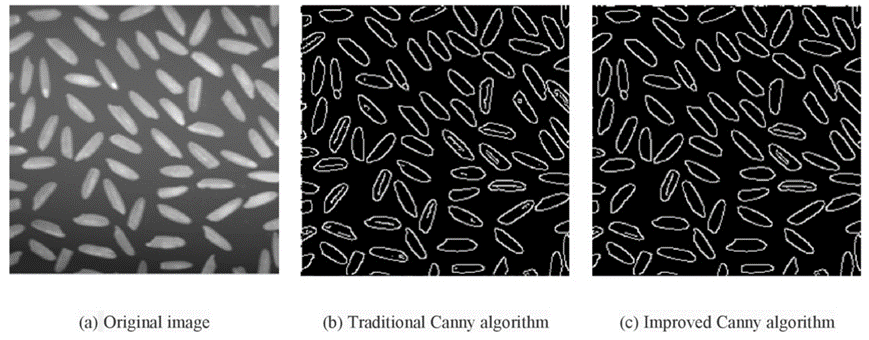
\includegraphics{2_1.png}
  \end{center}
  \caption[Poem]{หลักการทำงานของ Canny edge detection}
\end{figure}

ขั้นตอนหลักในการทำ Canny edge detection มีดังนี้:

\begin{itemize}
  \item {Gaussian Filter: เพื่อลด noise ไปจากภาพ ทำให้ไม่เกิดขอบภาพที่ไม่ต้องการ}
  \item {Prewitt หรือ Sobel edge detector: หา Edge strength และ Edge orientation}
  \item {Edge orientation Substituted: เปลี่ยนค่า orientation ของ edge ให้อยู่ในช่วงที่สามารถระบุพิกัดเป็นตำแหน่งของ pixel รอบๆได้}
\end{itemize}


\begin{figure}[h!]
  \begin{center}
    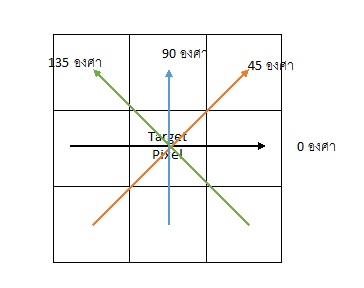
\includegraphics[height=7cm]{2_2.jpg}
  \end{center}
  \caption[Poem]{Edge orientation Substituted}
\end{figure}

\newpage
\begin{itemize}
  \item {Non-maximum Suppression}
\end{itemize}

\begin{figure}[h!]
  \begin{center}
    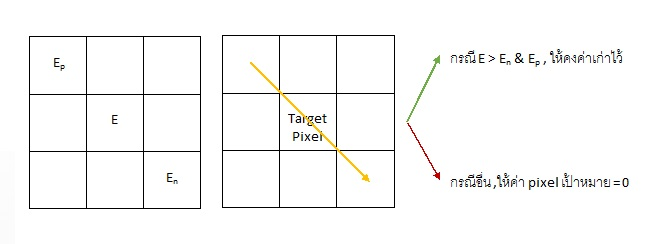
\includegraphics{2_3.jpg}
  \end{center}
  \caption[Poem]{Non-maximum Suppression}
\end{figure}

\begin{itemize}
  \item {Double threshold: เลือกค่าช่วง Edge strength ที่ต้องการแสดงไว้ และค่าที่ต่ำกว่าขอบเขตที่ระบุ ให้ค่า pixel นั้น = 0}
  \item {Hysteresis: แยกขอบออกเป็นส่วนๆ แบ่งตามตำแหน่งที่เชื่อต่อกันและความเข้ม ขอบที่มีความเข้มอ่อนจะไม่เชื่อมต่อกับขอบส่วนที่มีความเข้มสูง เราจะกำจัดส่วนนั้นทิ้งไป}
\end{itemize}

\newpage
\begin{figure}[h!]
  \begin{center}
    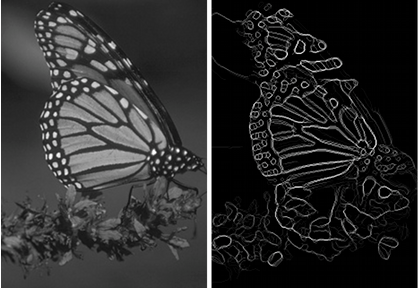
\includegraphics[height=8cm]{2_4.png}
  \end{center}
  \caption[Poem]{Hysteresis}
\end{figure}

\section{Active Contour}

เป็นเครื่องมือที่ใช้ในการตรวจจับและวาดเส้นขอบ (contour) ของวัตถุในภาพดิจิตอล โดยทั่วไปมักใช้ในการวาดเส้นขอบของวัตถุที่มีรูปร่างที่ไม่เป็นระเบียบหรือมีรูปร่างที่ซับซ้อน เช่น เครื่องตรวจจับเส้นขอบของลูกบอลในภาพถ่าย หรือการตรวจจับขอบของเซลล์ที่มีรูปทรงเป็นรูปเป็นระเบียบในภาพทางการแพทย์

\begin{figure}[h!]
  \begin{center}
    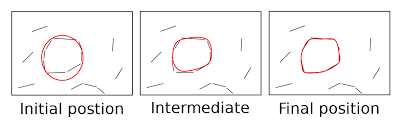
\includegraphics{2_5.png}
  \end{center}
  \caption[Poem]{หลักการทำงาน ของActive Contour}
\end{figure}

\newpage
\subsection{Active Contour : Snake Model}
เป็นโมเดลที่ใช้ใน Computer Vision สำหรับการวาดเส้นรอบวัตถุในภาพ 2 มิติ โมเดลนี้ถูกพัฒนาโดย \newline
Michael Kass, Andrew Witkin และ Demetri Terzopoulos ในปี 1987 โมเดล Snake เปรียบเสมือนเส้นยางยืดหยุ่นที่ถูกดึงดูดไปยังขอบของวัตถุในภาพ โมเดลจะใช้พลังงานสองประเภทในการดึงดูดเส้นยางไปยังขอบวัตถุ:

\begin{itemize}
  \item {พลังงานภายใน: ควบคุมความโค้งและความเรียบของเส้นยาง}
  \item {พลังงานภายนอก: ดึงดูดเส้นยางไปยังขอบของวัตถุในภาพ}
\end{itemize}

ในการนับรูปทรงต่างๆในภาพเราจะใช้  Snake Model ในการทำงานดังนี้:

\begin{enumerate}
  \item {กำหนดเส้นโค้งเริ่มต้น: เส้นโค้งเริ่มต้นสามารถกำหนดแบบสุ่ม หรือใช้ข้อมูลจากภาพ เช่น ขอบภาพ}
  \item {คำนวณพลังงาน: พลังงานจะถูกคำนวณจาก 3 องค์ประกอบ:}
  \begin{itemize}
  \item {พลังงานภายใน: วัดความเรียบของเส้นโค้ง}
  \item {พลังงานภาพ: วัดความสอดคล้องของเส้นโค้งกับภาพ}
  \item {พลังงานการเชื่อมต่อ: วัดความเชื่อมต่อของเส้นโค้ง}
  \end{itemize}
  \item {ปรับรูปร่างเส้นโค้ง: เส้นโค้งจะปรับรูปร่างของตัวเองเพื่อลดพลังงานรวม}
  \item {ทำซ้ำขั้นตอน 2 และ 3: ทำซ้ำจนกว่าเส้นโค้งจะลู่เข้า}
\end{enumerate}

\begin{itemize}
  \item {การนับรูปทรง:}
\end{itemize}

หลังจากเส้นโค้งลู่เข้าแล้ว จำนวนรูปทรงสามารถนับได้โดยการนับจำนวนเส้นโค้งที่แยกจากกัน

\begin{figure}[h!]
  \begin{center}
    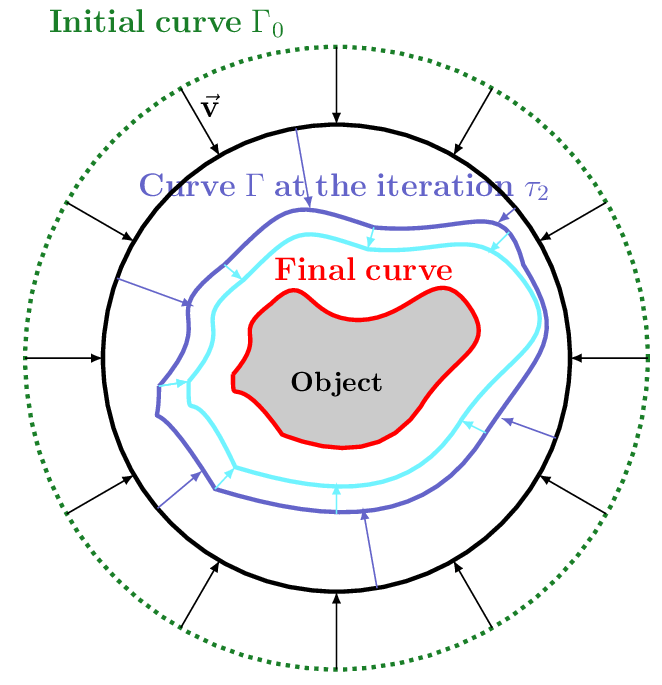
\includegraphics[height=8cm]{2_6.png}
  \end{center}
  \caption[Poem]{หลักการทำงานของ Active Contour : Snake Model}
\end{figure}

\section{\ifenglish%
Extracurricular knowledge used, applied, or integrated in this project
\else%
ความรู้นอกหลักสูตรซึ่งถูกนำมาใช้หรือบูรณาการในโครงงาน
\fi
}

\subsection{emulsion}

ระบบคอลลอยด์ (emulsion) ที่ประกอบด้วยเหลวตั้งแต่ 2 ชนิดขึ้นไป ซึ่งปกติไม่ผสมเป็นเนื้อเดียวกัน เช่น น้ำกับน้ำมัน ผสมรวมเป็นเนื้อเดียวกันได้โดยไม่แยกชั้น โดยของเหลวส่วนหนึ่งแตกตัวเป็นหยดเล็กๆ เรียกว่า วัฏภาคภายใน หรือส่วนที่กระจายตัว (internal or dispersed phase) ซึ่งจะกระจายตัวแทรกอยู่ในของเหลวอีกชนิดหนึ่ง เรียกว่า วัฏภาคภายนอก (external or continuous phase) ส่วนที่ต่อเนื่อง


อิมัลชันแบ่งเป็น 2 ประเภทหลัก คือ

\begin{itemize}
  \item {อิมัลชันชนิดน้ำมันในน้ำ (oil-in-water emulsion, O/W) มีน้ำมันเป็นวัฎภาคภายใน และน้ำเป็นวัฎภาคภายนอก เช่น น้ำนม (milk) ข้อสังเกตุ หรือวิธีทดสอบอิมัลชันประเภทนี้คือ สามารถทำให้เจือจางได้ด้วยการเติมน้ำ มีค่าการนำไฟฟ้า (electrical conductivity) สูงกว่า ผสมได้กับสีชนิดที่ละลายน้ำ (water soluble dye)}
  \item {อิมัลชันชนิดน้ำในน้ำมัน (water-in-oil emulsion, W/O) มีน้ำเป็นวัฎภาคภายใน และน้ำมันเป็นวัฎภาคภายนอก เช่น เนย (butter) มายองเนส (mayonnaise) น้ำสลัด (salad dressing) ไส้กรอก (sausage) ข้อสังเกตุ หรือวิธีทดสอบอิมัลชันประเภทนี้คือ สามารถทำให้เจือจางได้ด้วยการเติมน้ำมัน มีค่าการนำไฟฟ้า (electrical conductivity) ต่ำกว่า ผสมได้กับสีชนิดที่ละลายน้ำมัน (oil soluble dye)}
  \end{itemize}\

  \begin{figure}[h!]
    \begin{center}
      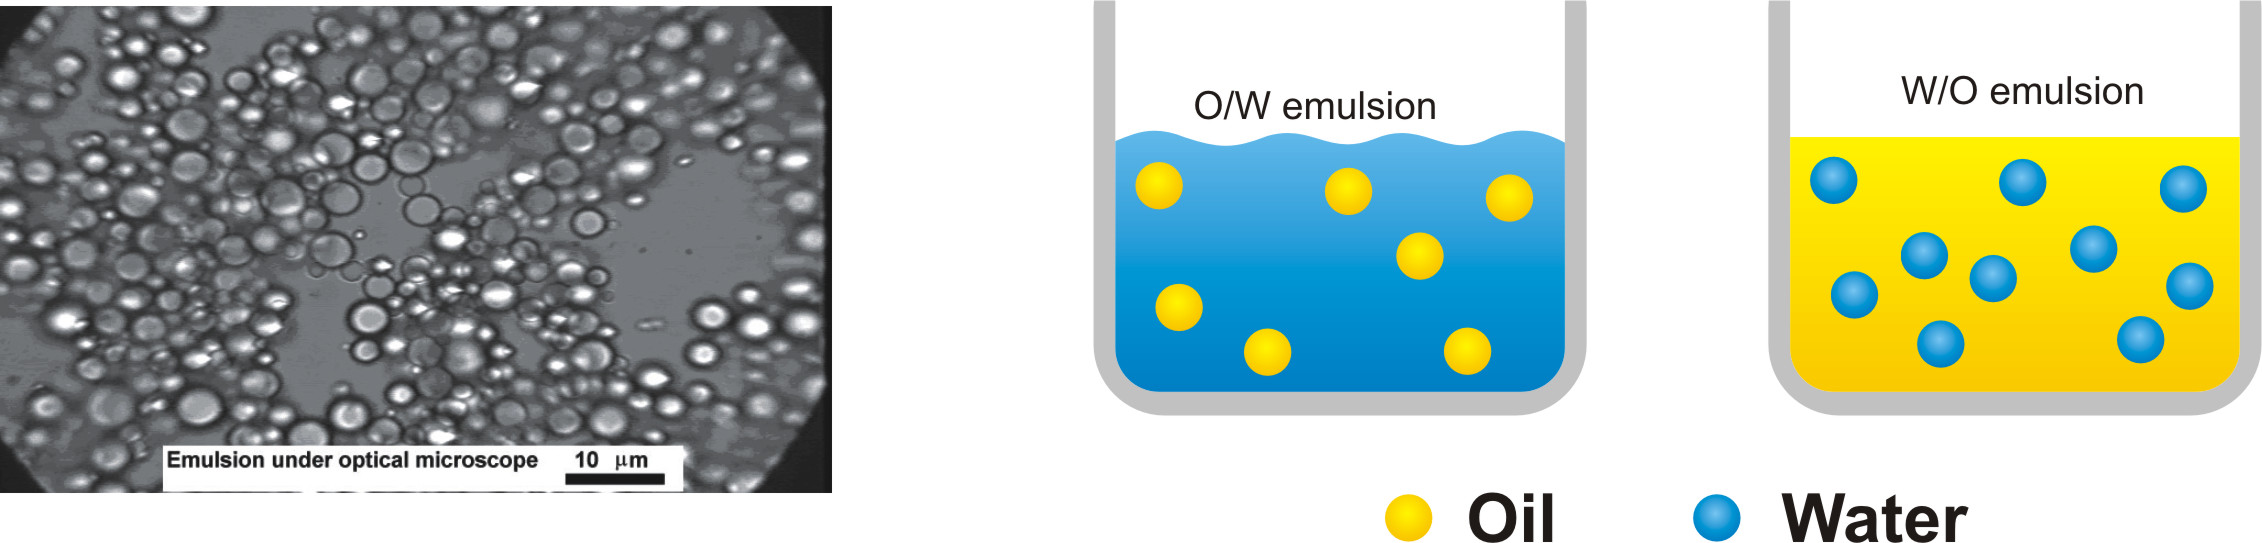
\includegraphics[width=\textwidth]{2_7.jpg}
    \end{center}
    \caption[Poem]{emulsion}
  \end{figure}

\chapter{\ifproject%
\ifenglish Project Structure and Methodology\else โครงสร้างและขั้นตอนการทำงาน\fi
\else%
\ifenglish Project Structure\else โครงสร้างของโครงงาน\fi
\fi
}


\makeatletter

% \renewcommand\section{\@startsection {section}{1}{\z@}%
%                                    {13.5ex \@plus -1ex \@minus -.2ex}%
%                                    {2.3ex \@plus.2ex}%
%                                    {\normalfont\large\bfseries}}

\makeatother
%\vspace{2ex}
% \titleformat{\section}{\normalfont\bfseries}{\thesection}{1em}{}
% \titlespacing*{\section}{0pt}{10ex}{0pt}

\section{โครงสร้างการทดลอง}

หลังจากกำหนดขอบเขตและหัวข้อโครงงาน และใช้แนวคิดการทดลองตามที่กลุ่มเราได้ว่าแผนกันโดยการขั้นตอนดังรูป ที่ 3.1

\begin{figure}[h!]
  \begin{center}
    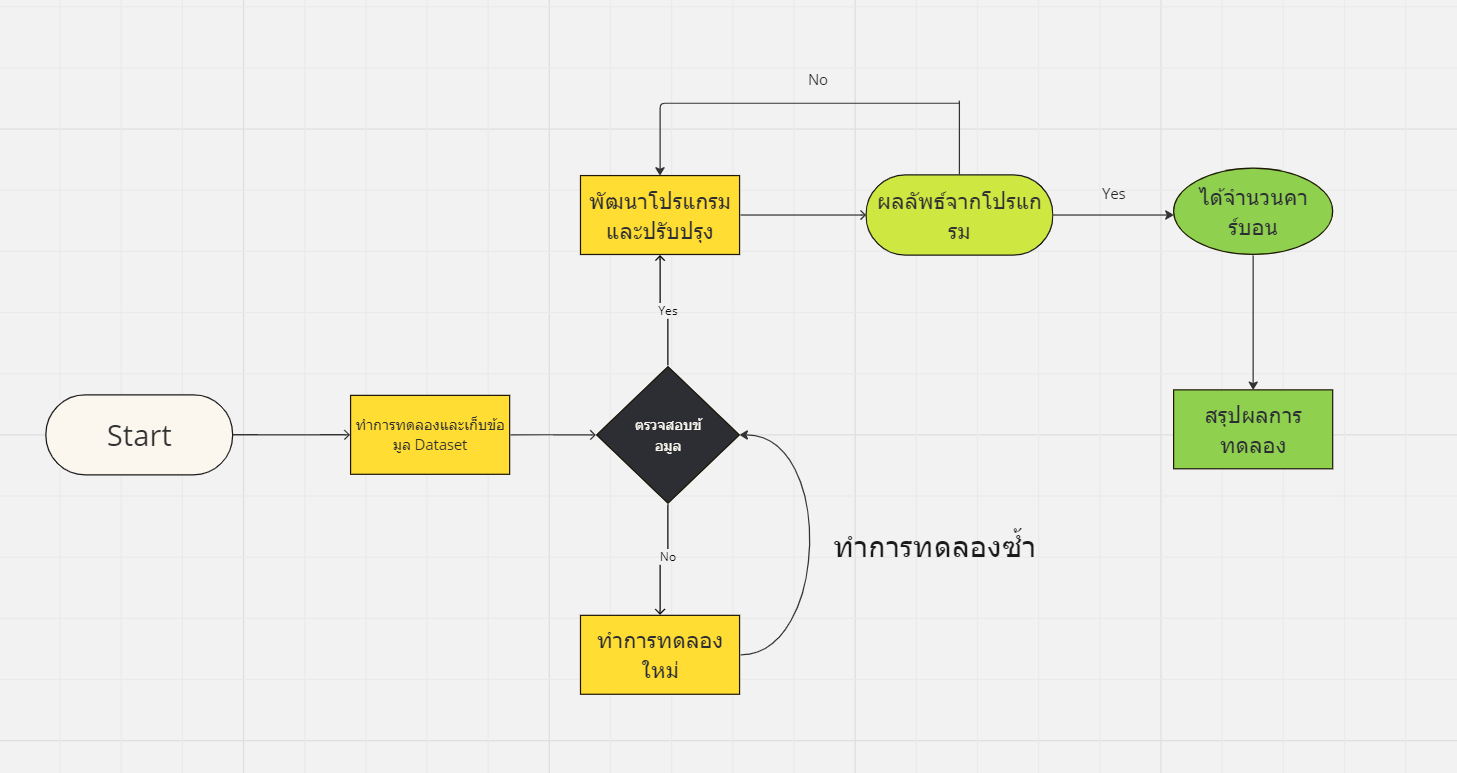
\includegraphics[width=\textwidth]{3_1.png}
  \end{center}
  \caption[Poem]{}
\end{figure}

\section{ขอบเขตการใช้งานระบบของผู้ใช้}

ระบบจะแบ่งผู้ใช้ออกเป็น 3 กลุ่มหลักๆ ได้แก่

\begin{enumerate}
  \item {อาจารย์ ครู}
  \item {บุคคลทั่วไปที่สนใจการทดลอง}
  \item {นักเรียน นักศึกษา}
\end{enumerate}

\subsection{อาจารย์ ครู}

\hspace{0.5 cm}โปรแกรมเราเหมาะสมสำหรับอาจารย์ หรือคุณครูที่กำลังสอนเกี่ยวกับการเกิดปฏิกิริยาอีมัลชั่นของก๊าซ \newline
คาร์บอน เพื่อจะแสดงจำนวนก๊าซคาร์บอนให้การทดลอง

\subsection{บุคคลทั่วไปที่สนใจการทดลอง}

\hspace{0.5 cm}บุคคลทั่วไปที่สนใจการทดลอง ที่สนใจในการทดลองหรือชอบความท้าทายในการทดลองเกี่ยวกับการผสม 
ก๊าซคาร์บอนกับก๊าซต่างๆ ในปฏิกิริยาอีมัลชั่น โดยสามารถนับจำนวนคาร์บอนที่มีรูปทรงต่างๆ จากโปรแกรมที่เราจะได้พัฒนาขึ้นมา

\subsection{นักเรียน นักศึกษา}

\hspace{0.5 cm}นักเรียน นักศึกษา ที่กำลังเรียนรู้เกี่ยวกับการเกิดอีมัลชั่นได้ โดยการผสมก๊าซคาร์บอนกับก๊าซต่างแล้วนับ จำนวนคาร์บอนที่เกิดขึ้นมาบันทึกเป็นกราฟทดลองได้ เช่นการทดลอง ก๊าซคาร์บอนกับก๊าซไนโตรเจน

ซึ่งขอบเขตการใช้งานระบบของผู้ใช้ อาจจะมีเพิ่มในภายหลัง ถ้ากลุ่มเราสามารถพัฒนาให้นับจำนวนก๊าซชนิดอื่นได้

\section{การเก็บข้อมูลการทดลอง และ การนับจำนวน}
หลังจากเราได้ทำการทดลองเสร็จแล้ว เราจะเก็บข้อมูลและนับจำนวนคาร์บอน ไม่ว่ารูปทรงจะเป็นอย่างไร \newline
ที่เราทดลองได้ ดังรูปตัวอย่างที่ 3.3

\begin{figure}[h!]
  \begin{center}
    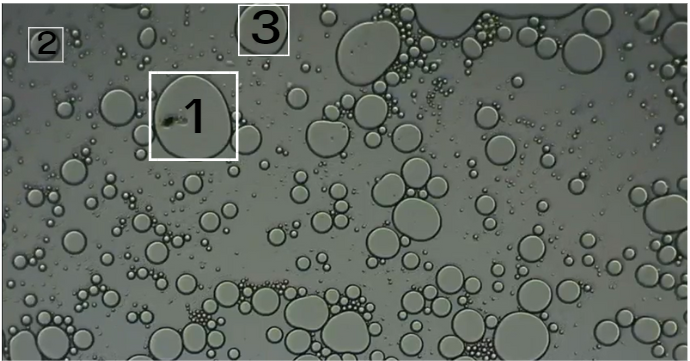
\includegraphics[width=\textwidth]{3_2.png}
  \end{center}
  \caption[Poem]{}
\end{figure}

\chapter{\ifproject%
\ifenglish Experimentation and Results\else การทดลองและผลลัพธ์\fi
\else%
\ifenglish System Evaluation\else การประเมินระบบ\fi
\fi}

การประเมินระบบของโครงงาน เพื่อวัดความสามารถและประเมินประสิทธิภาพของระบบ แบ่งออกเป็น 3 ส่วนหลักๆ ดังนี้

A. การประเมินและวัดผลกระบวนการนับจำนวนของฟองก๊าชคาร์บอนไดออกไซด์ที่เกิดขึ้น: ในส่วนนี้ เราจะใช้เทคโนโลยีการประมวลผลภาพเพื่อตรวจสอบและนับจำนวนของฟองก๊าชคาร์บอนไดออกไซด์ในพื้น ที่ที่สนใจ โดยใช้การวิเคราะห์ภาพเพื่อตรวจจับฟองก๊าช และนับจำนวนฟองก๊าชที่พบในภาพต่อหน่วยพื้นที่ เทคโนโลยีการประมวลผลภาพช่วยให้สามารถทำงานได้อย่างรวดเร็วและแม่นยำ

B. การประเมินและวัดผลความสามารถในการระบุขนาดของฟองก๊าชคาร์บอนไดออกไซด์ที่เกิดขึ้น: \newline
ในขั้นตอนนี้ เราจะใช้เทคโนโลยีการประมวลผลภาพเพื่อวัดและระบุขนาดของฟองก๊าชคาร์บอนไดออกไซด์ที่ตรวจจับได้ โดยการวัดเส้นผ่านศูนย์กลางของฟองก๊าชเพื่อกำหนดขนาดของฟองก๊าชได้อย่างที่ถูกต้องและแม่นยำ




C. การประเมินและระบุจำนวนประชากรของฟองก๊าชคาร์บอนไดออกไซด์ในพื้นที่: ในส่วนนี้ เราจะใช้เทคโนโลยีการประมวลผลภาพเพื่อประเมินและระบุจำนวนของฟองก๊าชคาร์บอนไดออกไซด์ในพื้นที่ที่สนใจ \newline
โดยการนับจำนวนฟองก๊าชคาร์บอนไดออกไซด์ทั้งหมดในพื้นที่และประเมินประชากรของฟองก๊าชคาร์บอน \newline
ไดออกไซด์ในพื้นที่นั้น


\ifproject
\include{chapters/conclusion}
\fi

\bibliography{sampleReport}

\ifproject
\normalspacing
\appendix
\include{chapters/appendix}

%% Display glossary (optional) -- need glossary option.
\ifglossary\glossarypage\fi

%% Display index (optional) -- need idx option.
\ifindex\indexpage\fi

\begin{biosketch}
\begin{center}
  \includegraphics[width=1.5in]{mugshot.jpg}
\end{center}
Your biosketch goes here. Make sure it sits inside
the \texttt{biosketch} environment.
\end{biosketch}
\fi % \ifproject
\end{document}
